% Drawing 154/02-24 -- folder 154, batch 02, archive page 37 (PDF page 38).
% Transcription: figure : deux pseudo-droites orange $D$, $D'$ se croisant sur une droite verte (pleine, doublée d'un pointillé), un petit segment foncé au point de croisement, une flèche vers le bas ; $\rightleftarrows$ ; la même figure, le croisement passé au-dessus de la droite verte, le petit segment foncé sur la droite entre les deux pseudo-droites
% Kind: crossing on a line, before and after. Method 2 (schematic redraw from the facsimile). Status: ok.
% Notes: Left: D and D' cross on the light green line (point computed), a short dark stroke at the crossing, light green dashes just above the line, a small arrow pointing down on the right. Middle: the two arrows, each with a bar at its tail. Right: the crossing lies above the line, the dark stroke is the piece of the line between the two strands. Redrawn 2026-11-12 (issue 128): to check again.
% Coordinates: 1 unit = 1 mm = 1/100 of the crop width (bbox in page fractions: [0.57, 0.295, 0.8, 0.355]).
% Redrawn by Claude (claude-fable-5-2), issue #128, 2026-11-12; not checked by a human; not compiled (no TeX in the session).
% Rights: reproduces part of the work -- behind RENDER_TRANSCRIPTS, never published by itself.
\documentclass[tikz,border=3pt]{standalone}
\usepackage{amsmath,amssymb}
\usetikzlibrary{patterns,arrows.meta}
\tikzset{Or/.style={orange!90!black}, Lg/.style={green!60!black!70}, pencil/.style={black!45}, struck/.style={black!35}, mpt/.style={circle,draw,inner sep=1.3pt}, pt/.style={circle,fill,inner sep=0.9pt}, opt/.style={circle,draw,fill=white,inner sep=1.1pt}}
\begin{document}
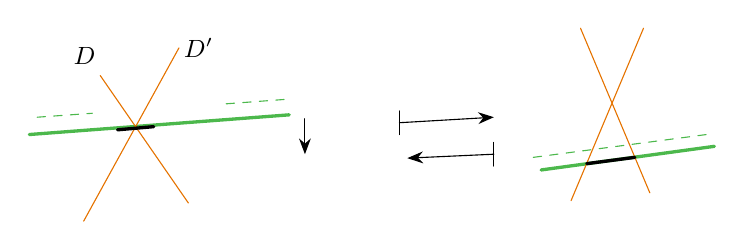
\begin{tikzpicture}[x=1mm,y=1mm,line cap=round,line join=round,font=\scriptsize]
\draw[Lg,very thick] (4,-23.5) -- (37,-21);
\draw[Lg,dashed] (5,-21.3) -- (12,-20.8);
\draw[Lg,dashed] (29,-19.6) -- (37,-19);
\draw[Or] (13,-16) -- (24.2,-32.2);
\draw[Or] (23,-12.5) -- (10.9,-34.5);
\draw[very thick] (15.2,-22.9) -- (19.8,-22.5);
\node[inner sep=1pt] at (11,-13.5) {\small $D$};
\node[inner sep=1pt] at (25.5,-12.5) {\small $D'$};
\draw[-{Stealth[length=2mm]}] (39,-21.5) -- (39,-26);
\draw[-{Stealth[length=2mm]}] (51,-22) -- (63,-21.3);
\draw (51,-20.5) -- (51,-23.5);
\draw[-{Stealth[length=2mm]}] (63,-26) -- (52,-26.5);
\draw (63,-24.5) -- (63,-27.5);
\draw[Lg,very thick] (69,-28) -- (91,-25);
\draw[Lg,dashed] (68,-26.4) -- (90,-23.5);
\draw[Or] (74,-10) -- (82.8,-30.9);
\draw[Or] (82,-10) -- (72.8,-31.9);
\draw[very thick] (80.9,-26.4) -- (74.8,-27.2);
\end{tikzpicture}
\end{document}
